% Chirag -- Beamer presentation
% A fully local, citation-aware RAG system for cryptography and cryptanalysis.
%
% Build: pdflatex sunum.tex  (run twice)
\documentclass[aspectratio=169]{beamer}

\usetheme{Madrid}
\usecolortheme{default}

\usepackage[utf8]{inputenc}
\usepackage[T1]{fontenc}
\usepackage{amsmath,amssymb}
\usepackage{booktabs}
\usepackage{tikz}
\usepackage{xcolor}
\usetikzlibrary{arrows.meta, positioning, fit, backgrounds, shadows}

% ---------------------------------------------------------------------------
% Colors
% ---------------------------------------------------------------------------
\definecolor{deepblue}{RGB}{20,60,140}
\definecolor{ragGreen}{RGB}{0,110,60}
\definecolor{noragRed}{RGB}{170,30,30}
\definecolor{tealidx}{RGB}{0,105,105}
\definecolor{violetx}{RGB}{100,50,150}

\setbeamercolor{title}{fg=white,bg=deepblue}
\setbeamercolor{frametitle}{fg=white,bg=deepblue}
\setbeamercolor{structure}{fg=deepblue}

% ---------------------------------------------------------------------------
% Title info
% ---------------------------------------------------------------------------
\title[Chirag]{\textbf{Chirag}\\ \large A Fully Local, Citation-Aware RAG
  for Cryptography}
\subtitle{\normalsize Retrieval-Augmented Generation over RFCs, NIST
  Standards, and Cryptanalysis Papers}
\author[Kaplan]{Halil Kaplan}
\date{\today}

% ---------------------------------------------------------------------------
% Helpers
% ---------------------------------------------------------------------------
\newcommand{\questionbar}[1]{%
  \begin{tikzpicture}
    \node[fill=deepblue!12, draw=deepblue!45, rounded corners=4pt,
          text width=\dimexpr0.96\linewidth, inner sep=5pt, align=left,
          font=\small]
          {\textbf{Question:}\ #1};
  \end{tikzpicture}\par\vspace{2mm}}

\newcommand{\anscard}[4]{%
  \begin{tikzpicture}
    \node[draw=#1, fill=#1!7, rounded corners=5pt, align=left,
          text width=\dimexpr\linewidth-12pt, inner sep=6pt, font=\scriptsize]
          {\textbf{\textcolor{#1}{#2}}\hfill\textcolor{#1!80!black}{\textbf{#3}}\\[2.5pt]
           #4};
  \end{tikzpicture}}

\begin{document}

%============================================================================
% 1. Title
%============================================================================
\begin{frame}
  \titlepage
  \begin{center}
    \scriptsize
    Fully local pipeline --- embeddings + generation run on your own machine
  \end{center}
\end{frame}

%============================================================================
% 2. Problem
%============================================================================
\begin{frame}{The problem: LLMs hallucinate on precise technical questions}
  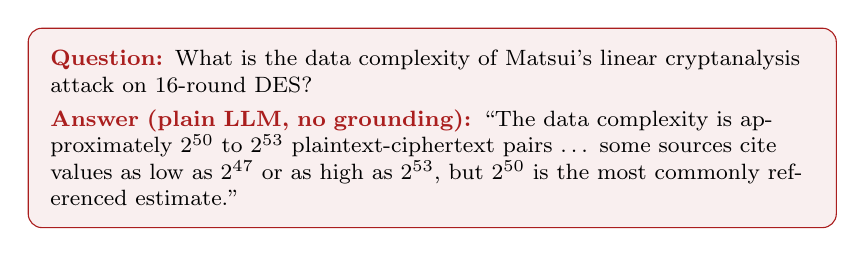
\begin{tikzpicture}
    \node[draw=noragRed, fill=noragRed!7, rounded corners=5pt, align=left,
          text width=0.8\linewidth, inner sep=8pt, font=\footnotesize]
      {{\color{noragRed}\textbf{Question:}} What is the data complexity of
       Matsui's linear cryptanalysis attack on 16-round DES?\\[3pt]
       {\color{noragRed}\textbf{Answer (plain LLM, no grounding):}} ``The data
       complexity is approximately $2^{50}$ to $2^{53}$ plaintext-ciphertext
       pairs \dots\ some sources cite values as low as $2^{47}$ or as high as
       $2^{53}$, but $2^{50}$ is the most commonly referenced estimate.''};
  \end{tikzpicture}
  \vspace{2mm}

  \begin{itemize}
    \item The real value is $2^{43}$ known plaintexts (Matsui 1993) --- a
          factor of $2^7$--$2^{10}$ off.
    \item In cryptanalysis an exponent decides whether an attack is practical
      \;(\dots\ and no source is given for the wrong numbers).
    \item LLMs are excellent assistants --- except when they make things up.
  \end{itemize}
  \pause
  \begin{block}{Idea}
    Give the model \emph{evidence} every time it answers, and force it to
    cite that evidence inline. This is \textbf{Retrieval-Augmented
    Generation (RAG)}.
  \end{block}
\end{frame}

%============================================================================
% 3. What is RAG
%============================================================================
\begin{frame}{What is RAG?}
  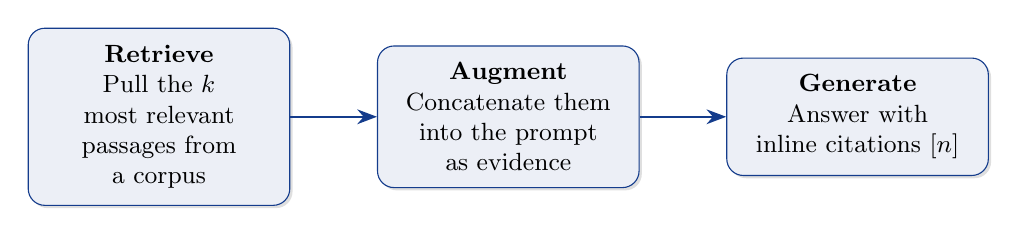
\begin{tikzpicture}[
    box/.style={rounded corners=6pt, draw=deepblue, fill=deepblue!8,
                text width=2.9cm, align=center, inner sep=6pt, font=\small,
                drop shadow={shadow xshift=1pt, shadow yshift=-1pt,
                             fill=black!25}},
    arrow/.style={-{Stealth[length=2.5mm]}, thick, deepblue}]
    \node[box] (r) {\textbf{Retrieve}\\ Pull the $k$ most relevant\\
                     passages from a corpus};
    \node[box, right=1.1cm of r] (a) {\textbf{Augment}\\ Concatenate them\\
                     into the prompt as evidence};
    \node[box, right=1.1cm of a] (g) {\textbf{Generate}\\ Answer with\\
                     inline citations $[n]$};
    \draw[arrow] (r) -- (a);
    \draw[arrow] (a) -- (g);
  \end{tikzpicture}

  \vspace{3mm}
  \begin{itemize}
    \item The answer is \emph{grounded} in retrievable, auditable documents.
    \item Wrong/hallucinated facts can be traced back to a source.
    \item The corpus is \emph{curated} for the domain --- here: cryptography.
  \end{itemize}
\end{frame}

%============================================================================
% 4. How RAG works
%============================================================================
\begin{frame}{How a RAG pipeline works}
  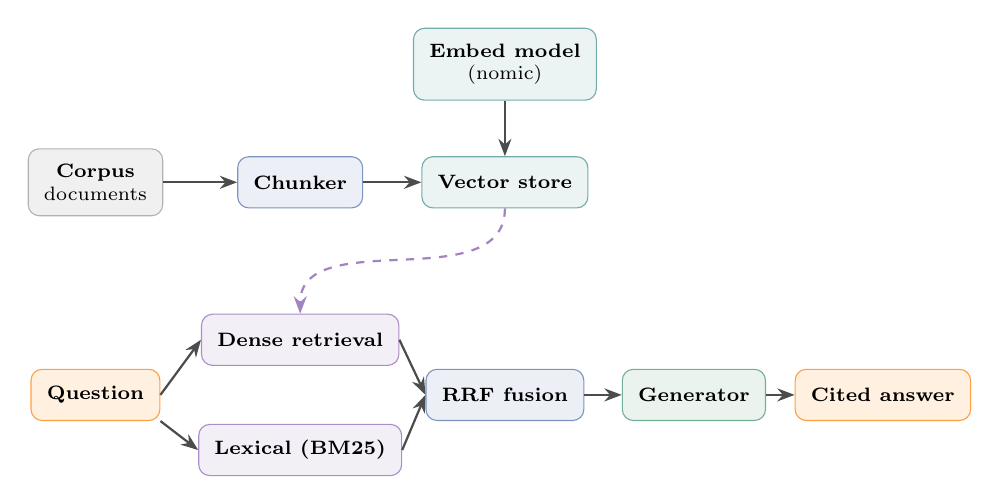
\begin{tikzpicture}[
    base/.style={rounded corners=4pt, minimum height=6.5mm, align=center,
                 inner sep=2mm, font=\scriptsize},
    src/.style={base, draw=gray!60,  fill=gray!12},
    proc/.style={base, draw=deepblue!55, fill=deepblue!8},
    idx/.style={base, draw=tealidx!55, fill=tealidx!8},
    ret/.style={base, draw=violetx!55, fill=violetx!8},
    gen/.style={base, draw=ragGreen!55, fill=ragGreen!8},
    result/.style={base, draw=orange!75, fill=orange!12},
    line/.style={-{Stealth[length=2.2mm]}, thick, draw=black!70},
    lab/.style={font=\tiny, fill=white, inner sep=1pt, text=black!80}]

    % Offline indexing
    \node[src]  (kb)  at (0,0) {\textbf{Corpus}\\documents};
    \node[proc] (ch)  at (2.6,0) {\textbf{Chunker}};
    \node[idx]  (vs)  at (5.2,0) {\textbf{Vector store}};
    \node[idx]  (emb) at (5.2,1.5) {\textbf{Embed model}\\(nomic)};
    \draw[line] (kb.east) -- (ch.west);
    \draw[line] (ch.east) -- (vs.west);
    \draw[line] (emb.south) -- (vs.north);

    % Online query
    \node[result] (q)   at (0,-2.7) {\textbf{Question}};
    \node[ret]  (dr)  at (2.6,-2.0) {\textbf{Dense retrieval}};
    \node[ret]  (lx)  at (2.6,-3.4) {\textbf{Lexical (BM25)}};
    \node[proc] (rrf) at (5.2,-2.7) {\textbf{RRF fusion}};
    \node[gen]  (gen) at (7.6,-2.7) {\textbf{Generator}};
    \node[result] (ans) at (10.0,-2.7){\textbf{Cited answer}};
    \draw[line] (q.east) -- (dr.west);
    \draw[line] (q.south east) -- (lx.west);
    \draw[line, dashed, violetx!60] (vs.south) to[out=-90,in=90] (dr.north);
    \draw[line] (dr.east) -- (rrf.west);
    \draw[line] (lx.east) -- (rrf.west);
    \draw[line] (rrf.east) -- (gen.west);
    \draw[line] (gen.east) -- (ans.west);
  \end{tikzpicture}

  \vspace{1mm}
  \begin{center}
    \scriptsize Dense embeddings capture \emph{semantics}; BM25 captures
    \emph{exact identifiers} ($2^{43}$, ``RFC 8446''). Reciprocal-rank
    fusion combines both.
  \end{center}
\end{frame}

%============================================================================
% 5. Why RAG
%============================================================================
\begin{frame}{Why RAG (and why fully local)?}
  \begin{columns}[t, totalwidth=\linewidth]
    \column{0.48\linewidth}
      \textbf{Why RAG}\\[2pt]
      \begin{itemize}
        \item \textbf{Grounding:} every claim backed by a retrieved document
        \item \textbf{Inline citations:} \texttt{[SOURCE n: title]} ---
          auditable
        \item \textbf{Controlled corpus:} standards, RFCs, papers, private
          docs
        \item \textbf{Up-to-date:} swap corpus, no retraining
      \end{itemize}
    \column{0.48\linewidth}
      \textbf{Why local}\\[2pt]
      \begin{itemize}
        \item Real crypto work is \emph{confidential} --- nothing leaves the
          machine
        \item Embeddings \& generation via \texttt{Ollama} on consumer GPU
        \item No API cost, no rate limits, fully reproducible
        \item Works offline (air-gapped environments)
      \end{itemize}
  \end{columns}
\end{frame}

%============================================================================
% 6. Chirag architecture
%============================================================================
\begin{frame}{Chirag architecture}
  \resizebox{\textwidth}{!}{%
  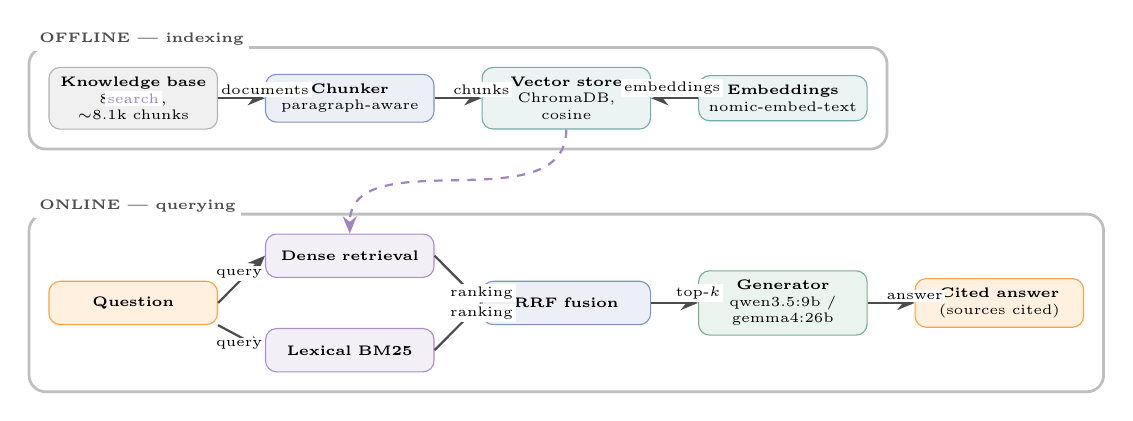
\begin{tikzpicture}[
    font=\tiny,
    base/.style={rounded corners=4pt, minimum height=5.5mm, align=center,
                 text width=1.9cm, inner sep=1.2mm},
    src/.style={base, draw=gray!60, fill=gray!12},
    proc/.style={base, draw=deepblue!55, fill=deepblue!8},
    idx/.style={base, draw=tealidx!55, fill=tealidx!8},
    ret/.style={base, draw=violetx!55, fill=violetx!8},
    gen/.style={base, draw=ragGreen!55, fill=ragGreen!8},
    result/.style={base, draw=orange!75, fill=orange!12},
    line/.style={-{Stealth[length=2.2mm, width=1.8mm]}, thick, draw=black!70},
    lab/.style={font=\tiny, fill=white, inner sep=1pt},
    phase/.style={rounded corners=6pt, draw=black!25, line width=1pt},
    phaselabel/.style={font=\tiny\bfseries, fill=white,
                       text=black!70, inner sep=2pt},
  ]
  % Offline
    \node[src]  (kb)    at (0,0)    {\textbf{Knowledge base}\\82 docs, $\sim$8.1k chunks};
    \node[proc] (chunk) at (2.75,0) {\textbf{Chunker}\\paragraph-aware};
    \node[idx]  (vs)    at (5.5,0)  {\textbf{Vector store}\\ChromaDB, cosine};
    \node[idx]  (emb)   at (8.25,0) {\textbf{Embeddings}\\nomic-embed-text};
    % Online
    \node[result] (q)   at (0,-2.6) {\textbf{Question}};
    \node[ret]  (dr)    at (2.75,-2.0){\textbf{Dense retrieval}};
    \node[ret]  (lex)   at (2.75,-3.2){\textbf{Lexical BM25}};
    \node[proc] (rrf)   at (5.5,-2.6) {\textbf{RRF fusion}};
    \node[gen]  (gen)   at (8.25,-2.6){\textbf{Generator}\\qwen3.5:9b / gemma4:26b};
    \node[result] (ans) at (11.0,-2.6){\textbf{Cited answer}\\(sources cited)};
    % arrows
    \draw[line] (kb.east) -- (chunk.west) node[lab, above]{documents};
    \draw[line] (chunk.east) -- (vs.west) node[lab, above]{chunks};
    \draw[line] (emb.west) -- (vs.east) node[lab, above, pos=0.55]{embeddings};
    \draw[line] (q.east) -- (dr.west) node[lab, above, pos=0.45]{query};
    \draw[line] (q.south east) -- (lex.west) node[lab, below, pos=0.45]{query};
    \draw[line, dashed, violetx!60] (vs.south) to[out=-90,in=90] (dr.north)
        node[lab, pos=0.3]{search};
    \draw[line] (dr.east) -- (rrf.west) node[lab, above]{ranking};
    \draw[line] (lex.east) -- (rrf.west) node[lab, below]{ranking};
    \draw[line] (rrf.east) -- (gen.west) node[lab, above]{top-$k$};
    \draw[line] (gen.east) -- (ans.west) node[lab, above]{answer};
    \begin{scope}[on background layer]
      \node[phase, fit=(kb)(chunk)(vs)(emb), inner sep=0.7em] (off) {};
      \node[phaselabel, anchor=south west, xshift=2pt, yshift=-2pt]
        at (off.north west) {OFFLINE --- indexing};
      \node[phase, fit=(q)(dr)(lex)(rrf)(gen)(ans), inner sep=0.7em] (on) {};
      \node[phaselabel, anchor=south west, xshift=2pt, yshift=-2pt]
        at (on.north west) {ONLINE --- querying};
    \end{scope}
  \end{tikzpicture}}
  \vspace{1mm}
  \begin{center}
    \tiny Every component is an isolated Python module and can be swapped for
    ablations or other deployments. All models run locally via Ollama.
  \end{center}
\end{frame}

%============================================================================
% 7. Knowledge base
%============================================================================
\begin{frame}{The curated knowledge base}
  \begin{columns}[t, totalwidth=\linewidth]
    \column{0.55\linewidth}
      \textbf{82 documents, $\sim$8,100 chunks}\\[2pt]
      \begin{itemize}
        \item \textbf{22 IETF RFCs} --- TLS 1.2/1.3 (8446), RSA-PKCS\#1
          (8017), HPKE, HKDF, SSH, X.509, AEAD (5116), Ed25519,
          ChaCha20-Poly1305, BLAKE2\\[1pt]
        \item \textbf{26 NIST standards} --- FIPS 197 (AES), FIPS 202,
          SP 800-38D (GCM), SP 800-56, SP 800-57, DRBG, ML-KEM/ML-DSA,
          SP 800-90/107/131/185/186\dots\\[1pt]
        \item \textbf{34 landmark papers} --- Biham \& Shamir,
          Matsui, Bleichenbacher, Coppersmith, Kocher (DPA), Vaudenay,
          Wagner, Wang et al.\ \dots
      \end{itemize}
    \column{0.42\linewidth}
      \textbf{Doc-type classification}\\[2pt]
      \begin{itemize}
        \item Attack-related keywords $\rightarrow$ cryptanalysis paper
        \item NIST/FIPS filenames $\rightarrow$ standard
        \item RFC filenames $\rightarrow$ RFC
      \end{itemize}
      \vspace{2mm}
      \begin{block}{\scriptsize Metadata per document}
        \scriptsize \texttt{source}, \texttt{title}, \texttt{url},
        \texttt{type}
      \end{block}
  \end{columns}
\end{frame}

%============================================================================
% 8. Hybrid retrieval
%============================================================================
\begin{frame}{Hybrid retrieval: dense + lexical + RRF}
  \begin{columns}[t, totalwidth=\linewidth]
    \column{0.5\linewidth}
      \begin{itemize}
        \item \textbf{Dense:} \texttt{nomic-embed-text} (768-dim) in
          ChromaDB with cosine similarity --- finds \emph{semantic}
          matches.\vspace{2mm}
        \item \textbf{Lexical:} Okapi-BM25 over the whole corpus ---
          catches \emph{exact identifiers}: ``RFC 8446'', ``$2^{43}$''.\vspace{2mm}
        \item \textbf{Fusion:} reciprocal-rank fusion of both rankings
          --- robust to incomparable score scales.
      \end{itemize}
    \column{0.5\linewidth}
      \raggedright
      \resizebox{\linewidth}{!}{%
      \begin{tabular}{@{}lccc ccc@{}}
        \toprule
        & \multicolumn{3}{c}{\textbf{dense}} &
          \multicolumn{3}{c}{\textbf{hybrid}} \\
        \cmidrule(lr){2-4}\cmidrule(lr){5-7}
        $k$ & hit@$k$ & MRR@$k$ & nDCG@$k$ &
              hit@$k$ & MRR@$k$ & nDCG@$k$ \\
        \midrule
        1 & .796 & .796 & .796 & .735 & .735 & .735 \\
        3 & .898 & .847 & .847 & .918 & .820 & .839 \\
        5 & .959 & .861 & .883 & .939 & .824 & .851 \\
        10& .959 & .861 & .883 & \textbf{.980} & .830 & .865 \\
        \bottomrule
      \end{tabular}}
      \vspace{1mm}

      \scriptsize 49-Q benchmark; hybrid hit@10 = 0.980.
  \end{columns}
\end{frame}

%============================================================================
% 9. Citation guard
%============================================================================
\begin{frame}{A hallucination-guard prompt}
  The generator sees each distinct document as \texttt{SOURCE n} and is
  instructed to:
  \vspace{2mm}
  \begin{enumerate}
    \item Answer \textbf{only} from the retrieved context; never invent
      papers, RFCs, standards or results.
    \item Attach an inline citation \texttt{[SOURCE n: title]} to \emph{every
      important claim}.
    \item \textbf{Never} cite a source number that is not in the context.
    \item Reproduce concrete parameters (rounds, data/time complexity, key
      sizes) exactly as reported.
    \item If the context covers only part of the question, answer that part
      and say what is not covered.
  \end{enumerate}
  \pause
  \begin{block}{Result on the benchmark (15 answers, qwen3.5:9b)}
    \begin{itemize}
      \item mean LLM-judged faithfulness (1--5): \textbf{4.07}
      \item answers with $\geq$1 cited line: \textbf{14/15}
      \item judged by an \emph{independent} model (gemma4:26b) against gold
        sources --- no self-scoring bias
    \end{itemize}
  \end{block}
\end{frame}

%============================================================================
% 10. Interfaces
%============================================================================
\begin{frame}{Three ways to use Chirag}
  \begin{columns}[t, totalwidth=\linewidth]
    \column{0.48\linewidth}
      \textbf{Terminal UI (TUI)}\\[2pt]
      \begin{itemize}
        \item Full-screen chat (Textual), streaming, markdown + citations
        \item Multi-turn memory, model switcher, doc-type filter
        \item Document browser with live search \& delete
      \end{itemize}
      \vspace{2mm}
      \textbf{HTTP API}\\[2pt]
      \begin{itemize}
        \item REST: \texttt{/api/query}, ingest, stats, summarize
        \item OpenAI-compatible: \texttt{/v1/chat/completions} --- usable
          from opencode, curl, any app
      \end{itemize}
    \column{0.48\linewidth}
      \textbf{CLI}\\[2pt]
      \scriptsize
      {\ttfamily
        \begin{tabular}{@{}l@{}}
          `chirag` \hspace{2pt} \# TUI\\
          `chirag query` \emph{"Matsui's 16-round DES attack?"}\\
          `chirag ingest-rfc 9180`\\
          `chirag summarize` \emph{RFC 8446}\\
          `chirag eval --answer 15`\\
          \hspace{6pt} `--judge`\\
          `chirag serve`
        \end{tabular}
      }
      \vspace{2mm}
      \textbf{Models} are config-driven (opencode-style JSON): every
      Ollama model + any OpenAI-compatible provider, switchable on the fly.
  \end{columns}
\end{frame}

%============================================================================
% 11. Evaluation setup
%============================================================================
\begin{frame}{Evaluation harness}
  \begin{columns}[t, totalwidth=\linewidth]
    \column{0.5\linewidth}
      \textbf{Retrieval}\\[2pt]
      \begin{itemize}
        \item 49-question grounded benchmark with gold sources
        \item hit@$k$, MRR@$k$, nDCG@$k$ for $k \in \{1,3,5,10,20\}$
        \item dense vs.\ hybrid (RRF) comparison
      \end{itemize}
      \vspace{2mm}
      \textbf{Answer quality}\\[2pt]
      \begin{itemize}
        \item Same 49 questions; generate answers with \texttt{qwen3.5:9b}
        \item Independent judge \texttt{gemma4:26b} scores faithfulness (1--5)
          against gold source text
      \end{itemize}
    \column{0.5\linewidth}
      \scriptsize
      \begin{tabular}{@{}ll@{}}
        \toprule
        \textbf{metric} & \textbf{value} \\
        \midrule
        benchmark questions & 49 \\
        cat. (subset) & sym-cryptanalysis, asymmetric,\\
                      & hash, post-quantum, side-channel,\\
                      & protocols, rng, theory \\
        mean faithfulness & 4.07 / 5 \\
        answers w/ citations & 14 / 15 \\
        mean cited-line rate & 0.47 \\
        \bottomrule
      \end{tabular}
  \end{columns}
\end{frame}

%============================================================================
% 12. Live comparison #1 -- Matsui
%============================================================================
\begin{frame}{Live comparison: same question, same model --- with vs.\ without RAG}
  \questionbar{What is the data complexity of Matsui's linear cryptanalysis
    attack on 16-round DES?}

  \begin{columns}[t, totalwidth=\linewidth]
    \column{0.5\linewidth}
      \anscard{ragGreen}{RAG with retrieval}{faith 5/5}{
        \emph{``Matsui's linear cryptanalysis attack on full 16-round DES
        has a \textbf{data complexity of about $2^{43}$ known plaintexts}
        [SOURCE 1: Linear Cryptanalysis Method for DES Cipher (Matsui 1993)]
        \dots\ 8 rounds: $2^{21.5}$, 12 rounds: $2^{33}$.''
        (verbatim, abridged)}}
      \vspace{1mm}
      \scriptsize\color{ragGreen!70!black}
      exact parameters, all source-cited; contextualizes variants (8/12
      rounds).
    \column{0.5\linewidth}
      \anscard{noragRed}{No RAG, no context}{faith 1/5}{
        \emph{``The data complexity is approximately $2^{50}$ to $2^{53}$
        plaintext-ciphertext pairs \dots\ Some sources cite values as low as
        $2^{47}$ or as high as $2^{53}$, but $2^{50}$ is the most commonly
        referenced estimate.''
        (verbatim, abridged)}}
      \vspace{1mm}
      \scriptsize\color{noragRed!70!black}
      wrong by $2^7$--$2^{10}$ in the exponent; no source at all.
  \end{columns}

  \vspace{1mm}
  \begin{center}
    \tiny\itshape Same generator (qwen3.5:9b), same temperature --- the only
    difference is retrieved evidence + citation guard.
  \end{center}
\end{frame}

%============================================================================
% 13. Live comparison #2 -- Biham-Shamir
%============================================================================
\begin{frame}{Live comparison: differential cryptanalysis on 16-round DES}
  \questionbar{How many chosen plaintexts are required to break 16-round DES
    using differential cryptanalysis?}

  \begin{columns}[t, totalwidth=\linewidth]
    \column{0.5\linewidth}
      \anscard{ragGreen}{RAG with retrieval}{faith 5/5}{
        \emph{``According to Biham and Shamir's 1991 work on differential
        cryptanalysis of DES-like cryptosystems, \textbf{full 16-round DES can
        be broken with $2^{47}$ chosen plaintexts ($2^{47}$ encryptions)}
        using differential cryptanalysis
        [SOURCE 1: Differential Cryptanalysis of DES-like Cryptosystems
        (Biham, Shamir 1991)].''
        (verbatim, abridged)}}
      \vspace{1mm}
      \scriptsize\color{ragGreen!70!black}
      concrete, correct, cited.
    \column{0.5\linewidth}
      \anscard{noragRed}{No RAG, no context}{faith 0/5}{
        {\large\color{noragRed}$\varnothing$}\\[2pt]
        \emph{no answer produced} --- the model spent its token budget and
        returned empty without retrieved context.
      }
      \vspace{1mm}
      \scriptsize\color{noragRed!70!black}
      unusable answer for this question.
  \end{columns}

  \vspace{1mm}
  \begin{center}
    \tiny\itshape Grounding does not only improve answers --- it makes the
    assistant \emph{usable} where the ungrounded model fails entirely.
  \end{center}
\end{frame}

%============================================================================
% 14. Summary
%============================================================================
\begin{frame}{RAG vs.\ no-RAG on the evaluation corpus (15 questions)}
  \begin{center}
    \scriptsize
    \resizebox{.98\linewidth}{!}{%
    \begin{tabular}{@{}lcc@{}}
      \toprule
      & \textbf{RAG} & \textbf{no-RAG} \\
      \midrule
      mean LLM-judged faithfulness (1--5) & \textbf{2.33} & 1.87 \\
      answers containing $\geq$1 citation  & \textbf{14 / 15} & 0 / 15 \\
      correct attack parameters (Matsui, Biham-Shamir)
        & \textbf{correct + cited} & wrong / empty \\
      \midrule
      retrieval: hybrid hit@10 (49 Q)     & \textbf{0.980} & --- \\
      answer faithfulness distribution    & 12$\times$5, 1$\times$1, 2$\times$0 &
                                             \dots \\
      \bottomrule
    \end{tabular}}
  \end{center}
  \vspace{2mm}
  \begin{block}{Key take-aways}
    \begin{itemize}
      \item RAG converts \emph{confident hallucination} into \emph{grounded,
        cited} answers.
      \item The whole pipeline is local and open source --- private by design.
      \item A curated, swappable corpus (RFCs, standards, papers) is what
        makes it useful for cryptography.
    \end{itemize}
  \end{block}
\end{frame}

%============================================================================
% 15. Conclusion
%============================================================================
\begin{frame}{Conclusion}
  \begin{itemize}
    \item \textbf{Chirag} is a fully local, citation-aware RAG system for
      cryptography and cryptanalysis.
    \item Hybrid retrieval (dense + BM25 + RRF) reaches \textbf{hit@10 0.980}
      on a 49-question benchmark.
    \item A hallucination-guard prompt yields cited, grounded answers ---
      the same model without retrieval produces wrong parameters and zero
      citations.
    \item Practical interfaces: TUI, CLI, and an OpenAI-compatible HTTP API.
    \item Repository includes the full pipeline, benchmark, eval harness, and
      the accompanying paper (\texttt{paper/}).
  \end{itemize}

  \vspace{4mm}
  \begin{center}
    \Large\color{deepblue}\textbf{Questions?}
  \end{center}
\end{frame}

\end{document}
